\section{\texorpdfstring{Maticovy popis grafu, det, kostry}{Maticovy popis grafu, det, kostry}}
\vspace{5mm}
\large

\begin{definition}
Matice sousednosti grafu G
\end{definition}

\begin{theorem}[Pocet sledu]
Pro kazdy graf G a kazde prirozene cislo k obsahuje k-ta mocnina matice sousednosti A pocty sledu delky k mezi vrcholy grafu G, konkretne\\
$(A^k)_{a,b} = $ \# sledu delky k mezi a - b v G.
\end{theorem}
\begin{proof}
Indukci podle k.
\begin{enumerate}
	\item k = 0, sledy delky 0, neboli $ u - u $. Coz odpovida dle definice $ A^0 = I $.
	\item k = 1. Sled je prave hrana.
	\item indukcni krok:
	\[(A^{k+1})_{a,b} = (A^k * A)_{a,b} = \sum_{w \in V} (A^k)_{a,w} * A_{w,b} = \]
	na pozice $ (w,b) $ je 1 pokud existuje takova hrana, jinak 0. Proto
	\[ = \sum_{w, bw \in E} (A^k)_{a,w} = \]
	Dle I.P. se rovna poctu sledu delky k mezi $a - w$.
	Pak mezi vrcholy $ a - w $ existuje sled delky k. Rozdelime sledy dle konecneho vrcholu, ktery je soused $b$. Kazdy z techto sledu jednoznacne prodlouzime na sled delky $(k+1)$ do vrcholu b. Z toho predchozi soucet je prave \# pocet sledu delky $(k+1)$ mezi $ a - b $.
\end{enumerate}
\end{proof}

\begin{definition}
	$ L^{(n)}_G $ se dostane tak, ze vyskrtneme n-ty radek a slopec z Laplaceove matice.
\end{definition}
\begin{lemma}
\[ \forall w \subseteq E, |w| = n - 1: det((D^{(u)}_G)_w) = \twopartdef{0}{(V, w) \neq tree}{\pm 1}{ (V,w) = tree}  \]
\end{lemma}
\begin{proof}
	1) Necht $w \subseteq E$ je kostra. Pak je stromem $\Rightarrow$ ma list $v_1$. Premistime radek odpovidajiici $v_1$ do prvniho radku. Necht $e_1$ je hrana $v_1 - v_t$. Dame ji do prvniho sloupce.
	Pak na pozice (0,0) je $\pm 1$. Taky prvni radek je $(\pm 1, 0, ... 0)$ protoze vrhol je list.

	Odtranime $v_1$, necht $v_2$ je dalsi list a $e_2$ jeho hrana. Pak druhy radek je $(??, \pm 1, 0, ... 0)$. Tak pokracujeme dal.

	Muze se ale stat, ze dalsi vrhol je $u$ ktery jsme zrovna odstranili. Pouzijeme tvrzeni, ze strom ma aspon 2 listy. Pak muzeme vzit nejaky dalsi vrhol. Po ukonceni premistovani dostaneme $\pm 1$ na diagonale. Nad diagonalou same 0 $\Rightarrow det = \pm 1$. Premistenim jsme menili znamenko $det$. Ale $det^2 = 1$.

	2) Mame graf $w \subseteq E, |w| = |V| - 1$ ktery neni strom $\Rightarrow$ neni souvisly $\Rightarrow$ ma aspon 2 komponenty souvislosti. $V = V_1 \mathbin{\dot{\cup}} V_2$.
	BUNO $u \in V_2$. Pak z $V_1$ do $V_2$ nevede zadna hrana, cast matice je 0. Pak soucet radku odpovidajici $V_1, E(V_2)$ a $V_2, E(V_1)$ je 0 $\Rightarrow$ rakdy jsou LZ a det je 0.

	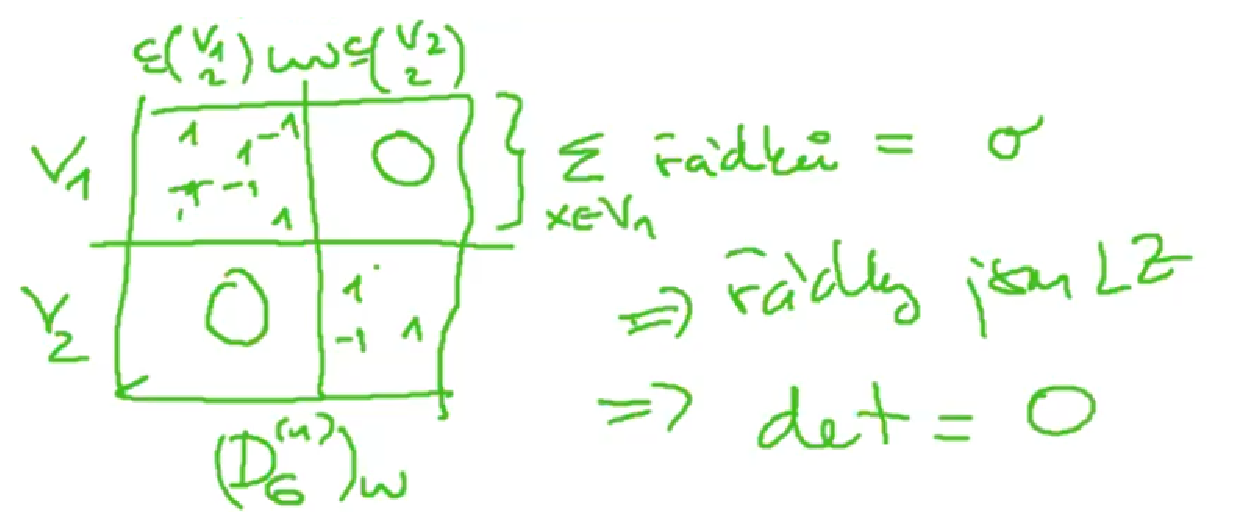
\includegraphics[scale=0.3]{kostra_lemma.eps}
\end{proof}

\begin{theorem}[Pocet koster]
	$ det(L^{(n)}_G) = $ \# koster grafu G
\end{theorem}
\begin{proof}
	Vezmeme matice incidence $ I_G $ (jenom 2 jednicky ve sloupci, v radku \# 1 je $deg(v)$), v kazdem jejim sloupci nahradime jednu jednicku hodnotou $(-1)$. Vyslednou matici oznacme $D_G$.

	$ I_G * I_G^T = $ skal. soucin radku i, j. Na diagonale $deg(v)$, mimo diag. 1 pro hrany, 0 - nehrany.

	Zmenime prave jednu 1ku ve kazdem sloupci na $-1$ (tim dostaneme orient. graf).
	\[ D_g * D_G^T = L_G \]
	Rovnost plati protoze skalarni soucin stejneho radku da $deg(v)$ jelikoz $ -1 * -1 = 1 $. Pokud nasobime ruzne radky, prislusne vrcholy nejsou spojene hranou - 0. Jinak maji prave 1 spolecnou pozici a dostaneme $-1 * 1 = -1$.

	Pak $det(L^{(u)}_G)$ spocitame jako $det(D^{(u)}_G * (D^{(u)}_G)^T)$

	Pouzijeme Cauchy-Benet formulu (det souciny obdelnikovych matic)
	\[ det(A*B) = \sum _{\substack{ w \subseteq {1,2, ..., n} \\ |w| = k}} det A_w * det B^w \]
	Kde $ A_w $ jsou n sloupcu matice A, $ B^w $ - n radku matice B.

	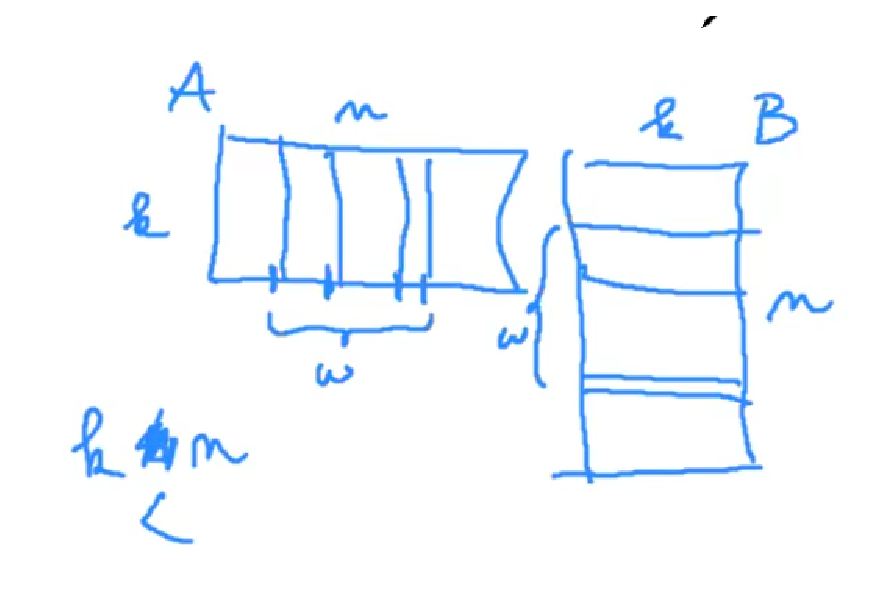
\includegraphics[scale=0.3]{cauchy-benet.eps}

	\[ det L^{(u)}_G = \sum_{\substack{w \subseteq E \\ |w| = n-1}} det(D^{(u)}_G) * (D^{(u)}_G)^{T} = \]
	Pro kazdou matici $ det A = det A^T $, pak
	\[ = \sum_{\substack{w \subseteq E \\ |w| = n-1}} det(D^{(u)}_G)^2 \]

	Kostra musi mit $(n-1)$ vrcholu; v det se divame na vsechny podmoziny hran $|w| = n - 1$.
	Ptame se jestli je strom. Proto suma nehore je prave
	\[ \sum_{\substack{w \\ (V,w) je \ kostra}} 1 \]
	Coz je \# koster G


\end{proof}
